\chapter{Experiments and Data Collection}\label{chapter:expt-data-collection}

\section{Sleep Experiments and Video Recordings}
We developed a custom imaging setup to perform high-resolution characterization of sleep-related behaviors in flies.
A custom 3D printed chamber (7.2X4.3X2.4 mm [WxHxL]) is placed in front of a IR sensitive (Flir) camera with telecentric lens (Edmund Optics).

\begin{figure}[ht!]
	\centering
	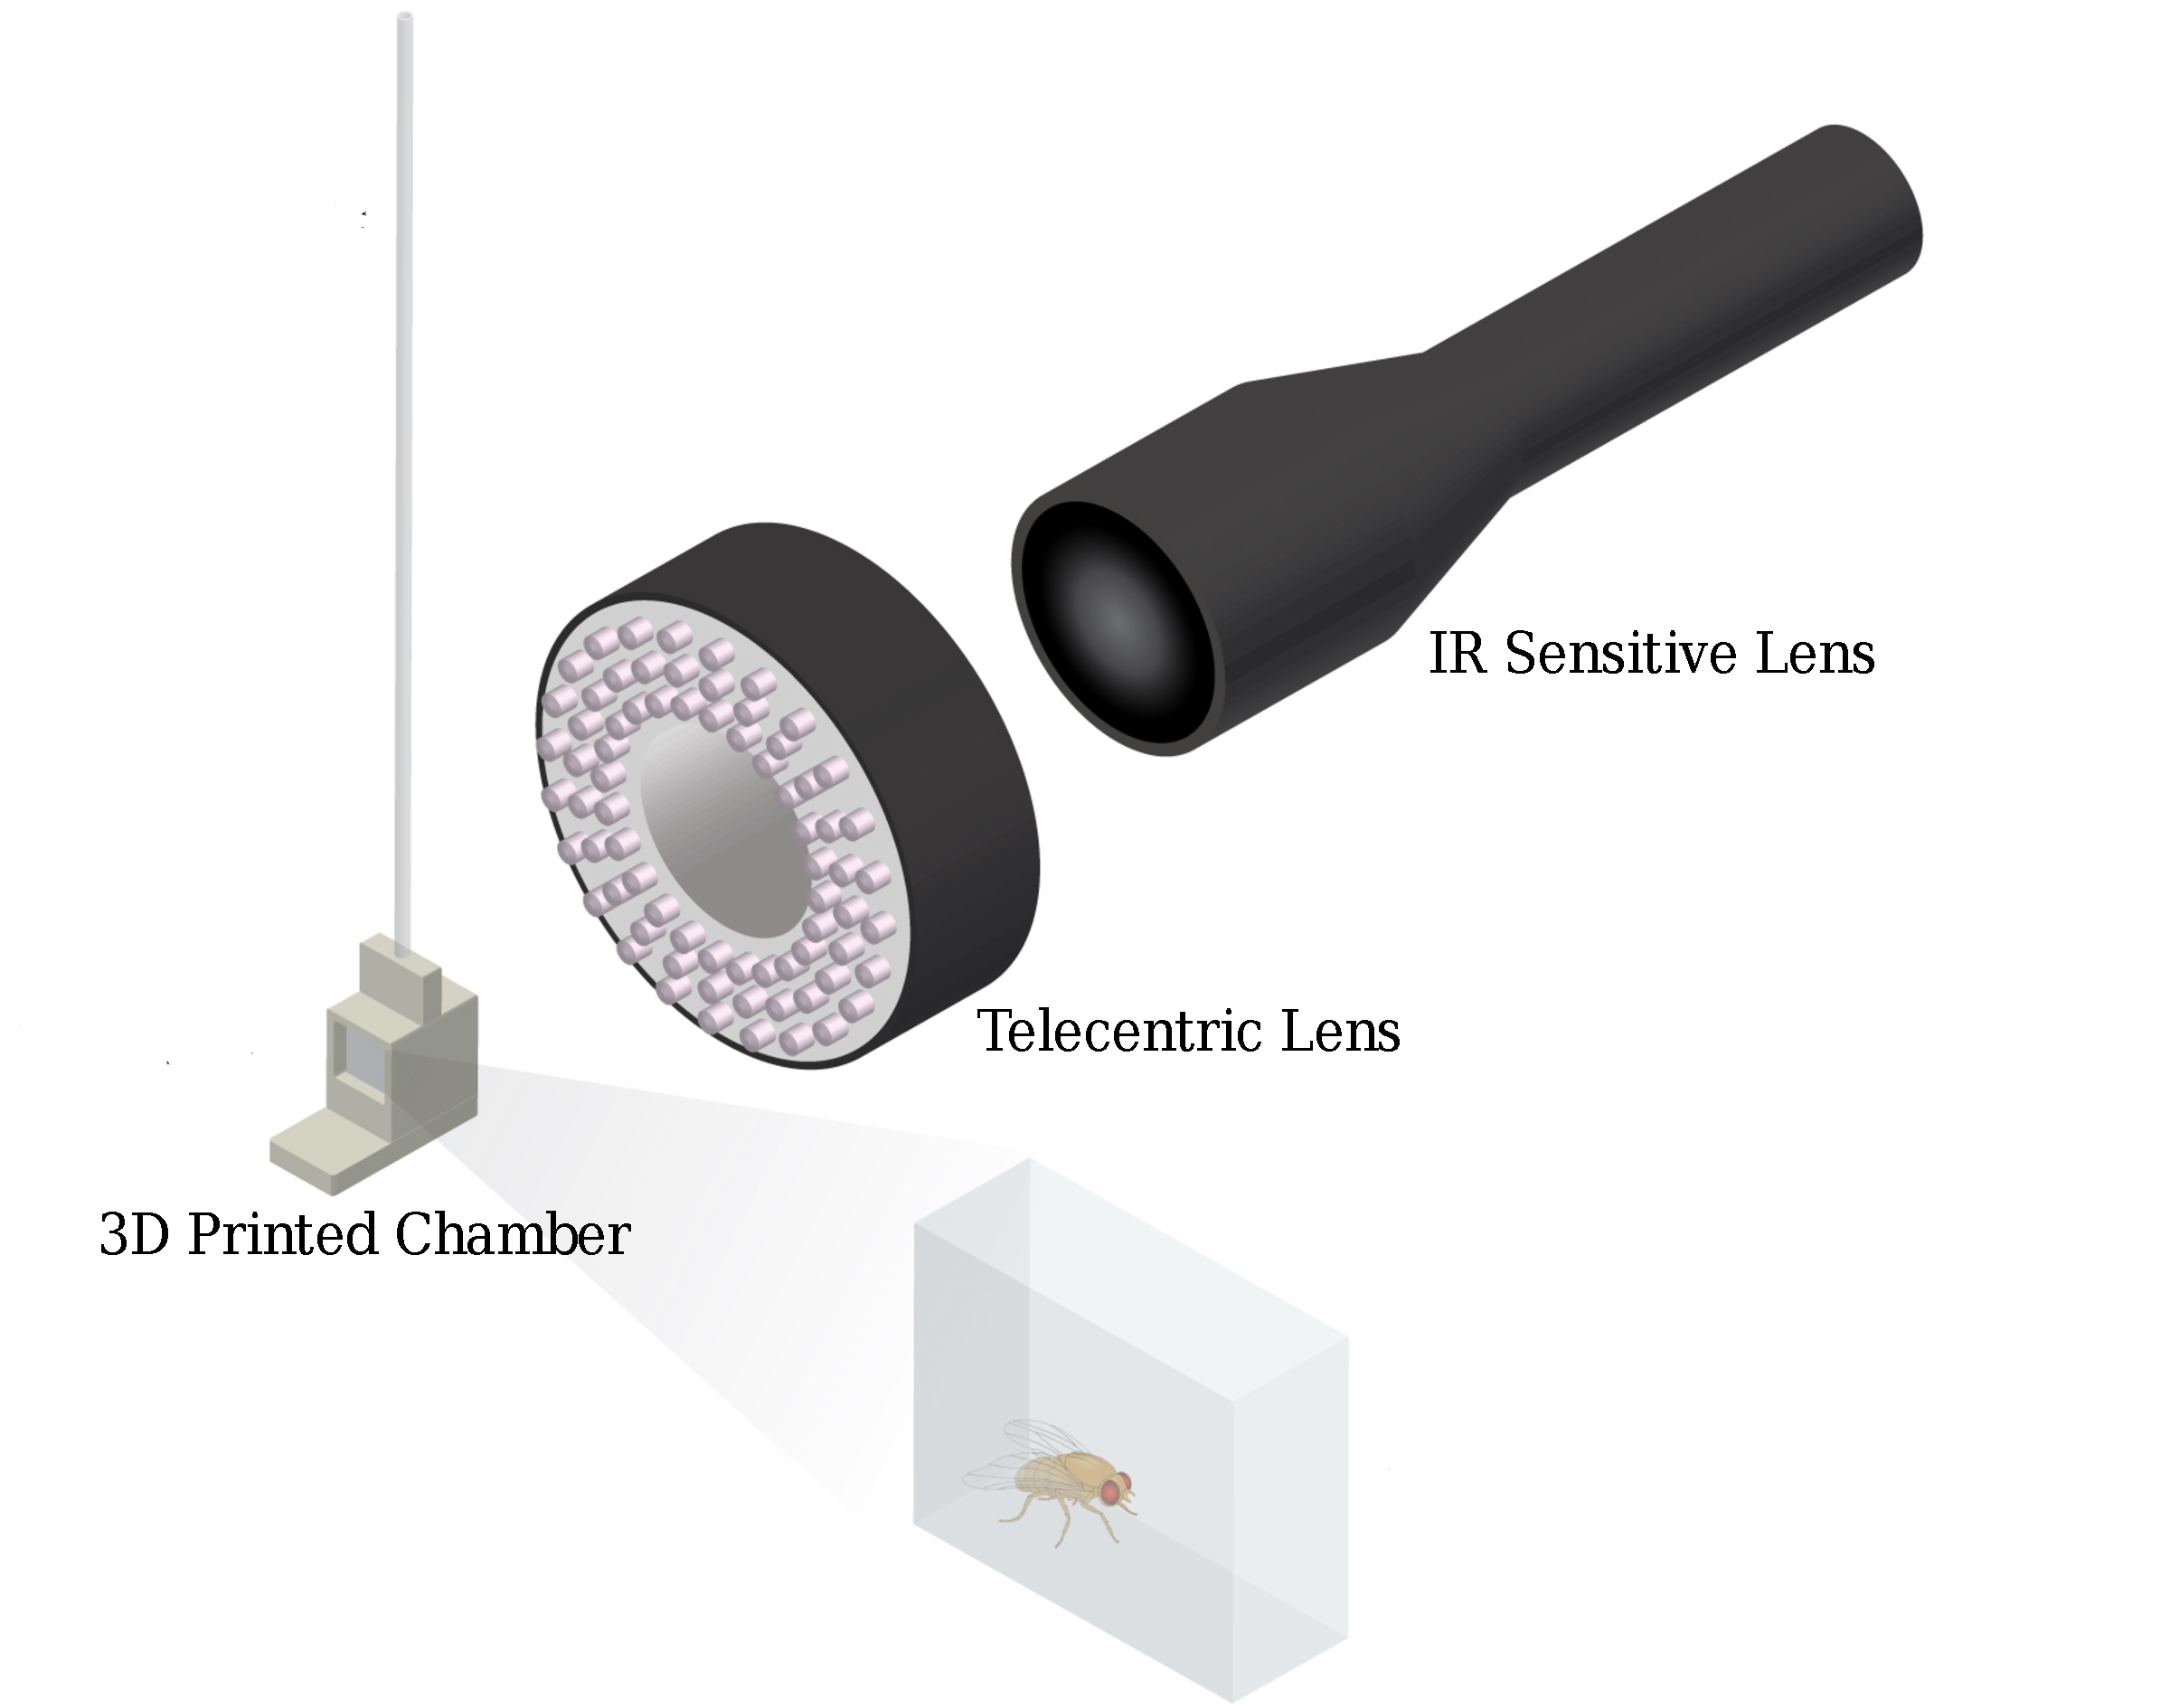
\includegraphics[width=0.75\linewidth]{figures/ExperimentalSetup.pdf}
	\caption[An illustration of the experimental setup which is used to perform high-resolution imaging of experiments.]{An illustration of the experimental setup which is used to perform high-resolution imaging of experiments.}
\end{figure}

Flies recorded from ZT10-ZT2 (16 hours) total.
Each chamber has a food port (1.5mm diameter) that allows access to liquid food (2.5\% yeast, 2.5\% sugar).
Recording setup is in light tight box and humidity control (60\%) is achieved via humidifier plugged into a humidity control switch.
Experimental flies are loaded to individual chambers at ZT8-ZT9 via mouth pipette or a small vacuum pump.
Individual chambers are sealed with a 7x7 mm acrylic windows.
Windows are coated with SigmaCote to prevent flies from ventral or dorsal postural positions.
5-7 day old female and male flies are used in the experiments.

\section{Pose Estimation and Tracking}

\begin{figure}[ht!]
	\centering
	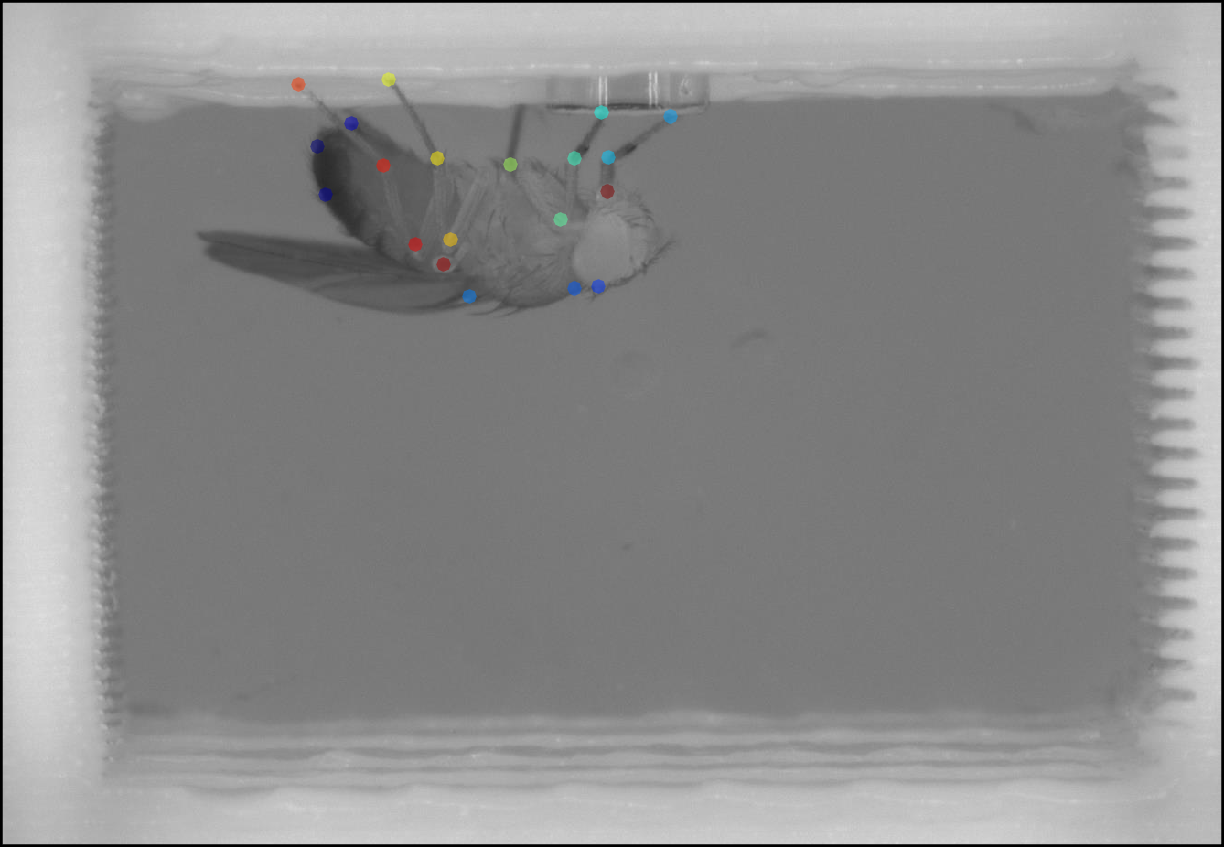
\includegraphics[width=0.75\linewidth]{figures/FlyTrackedBodyParts.png}
	\caption[An example frame of the fruit fly placed in 3D printed chamber.]{An example video recording frame of the fruit fly placed in 3D printed chamber. Colorful markers indicates the tracked body parts.}
\end{figure}

\section{Behavior Annotations}
3 annotators labeled 5 different behaviors (feeding, grooming, moving, haltere switch, proboscis pumping) across 11 videos (14 hours and 16 hours each, respectively for 7 wild type sleep experiments and 4 sleep deprivation experiments).
A single experiment is annotated by all 3 annotators to check rigor and overlap among annotators.
90\% coverage is required among annotators to proceed with annotation of a novel fly.

\begin{figure}[ht!]
	\centering
	\begin{subfigure}[ht!]{0.95\linewidth}
		\centering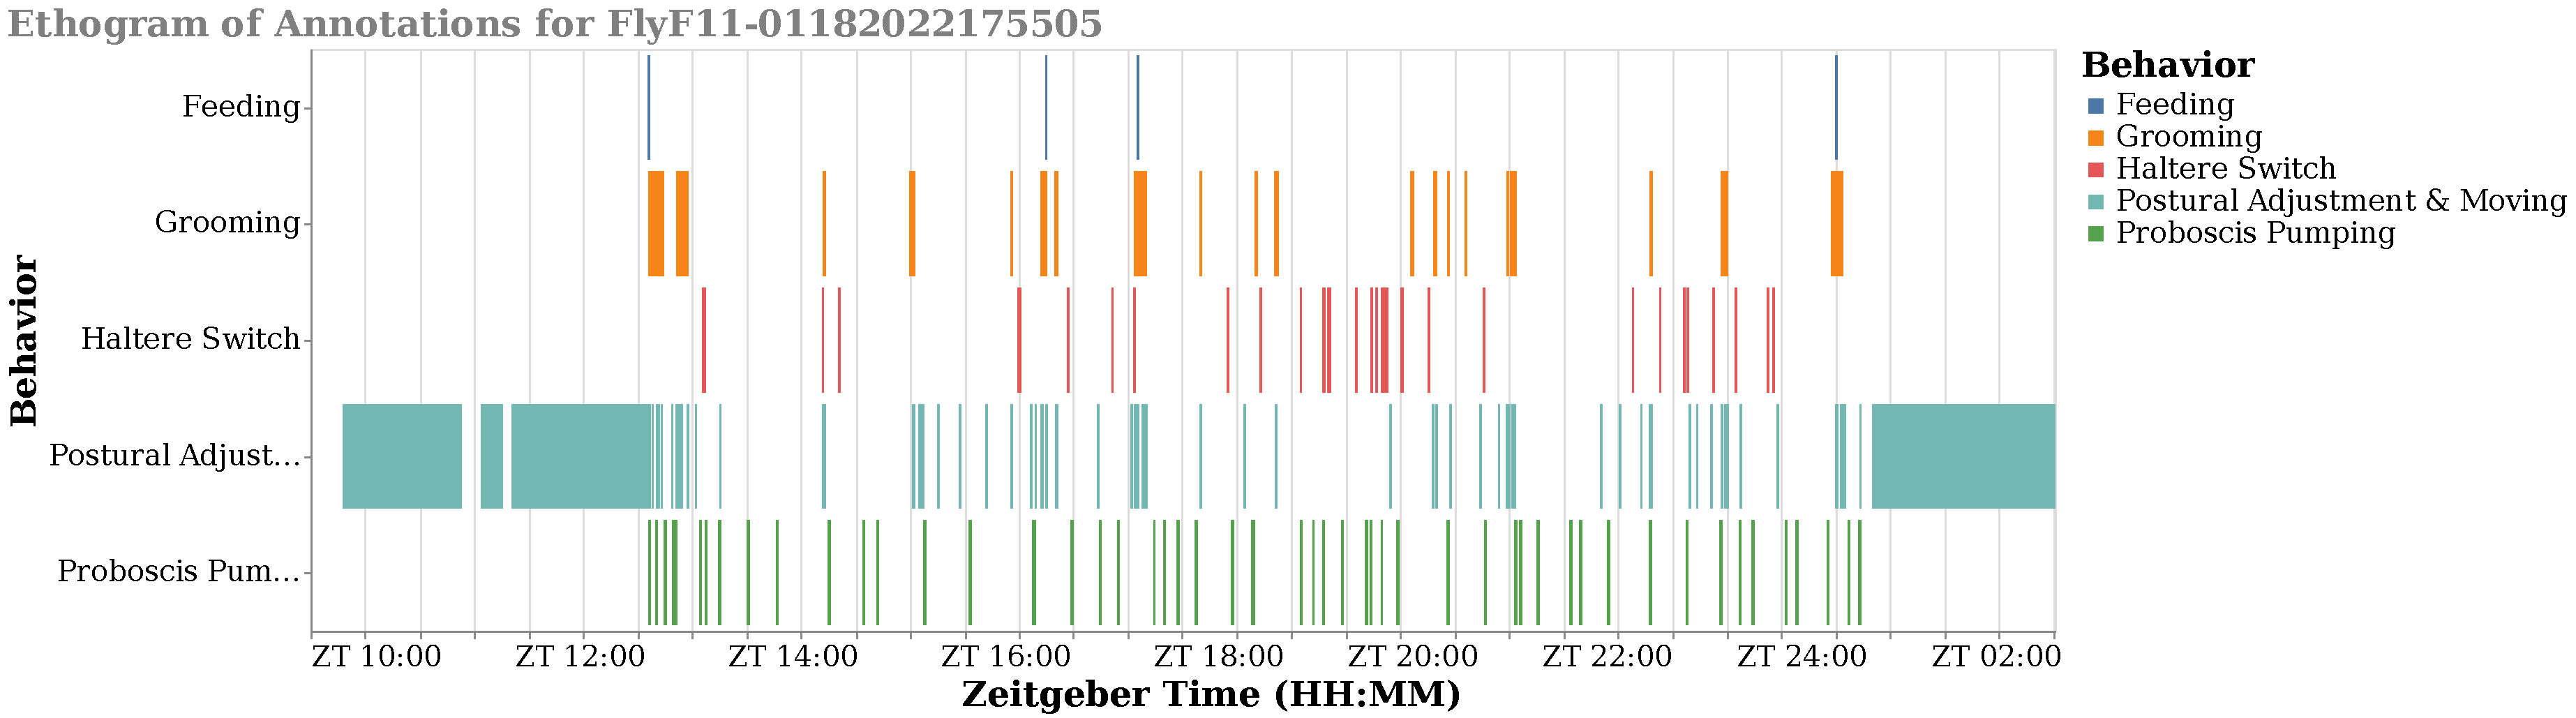
\includegraphics[width=\linewidth]{figures/FlyF11-01182022175505_annotation_ethogram.pdf}
		\caption{Wild type.}
	\end{subfigure}%

	\centering
	\begin{subfigure}[ht!]{0.95\linewidth}
		\centering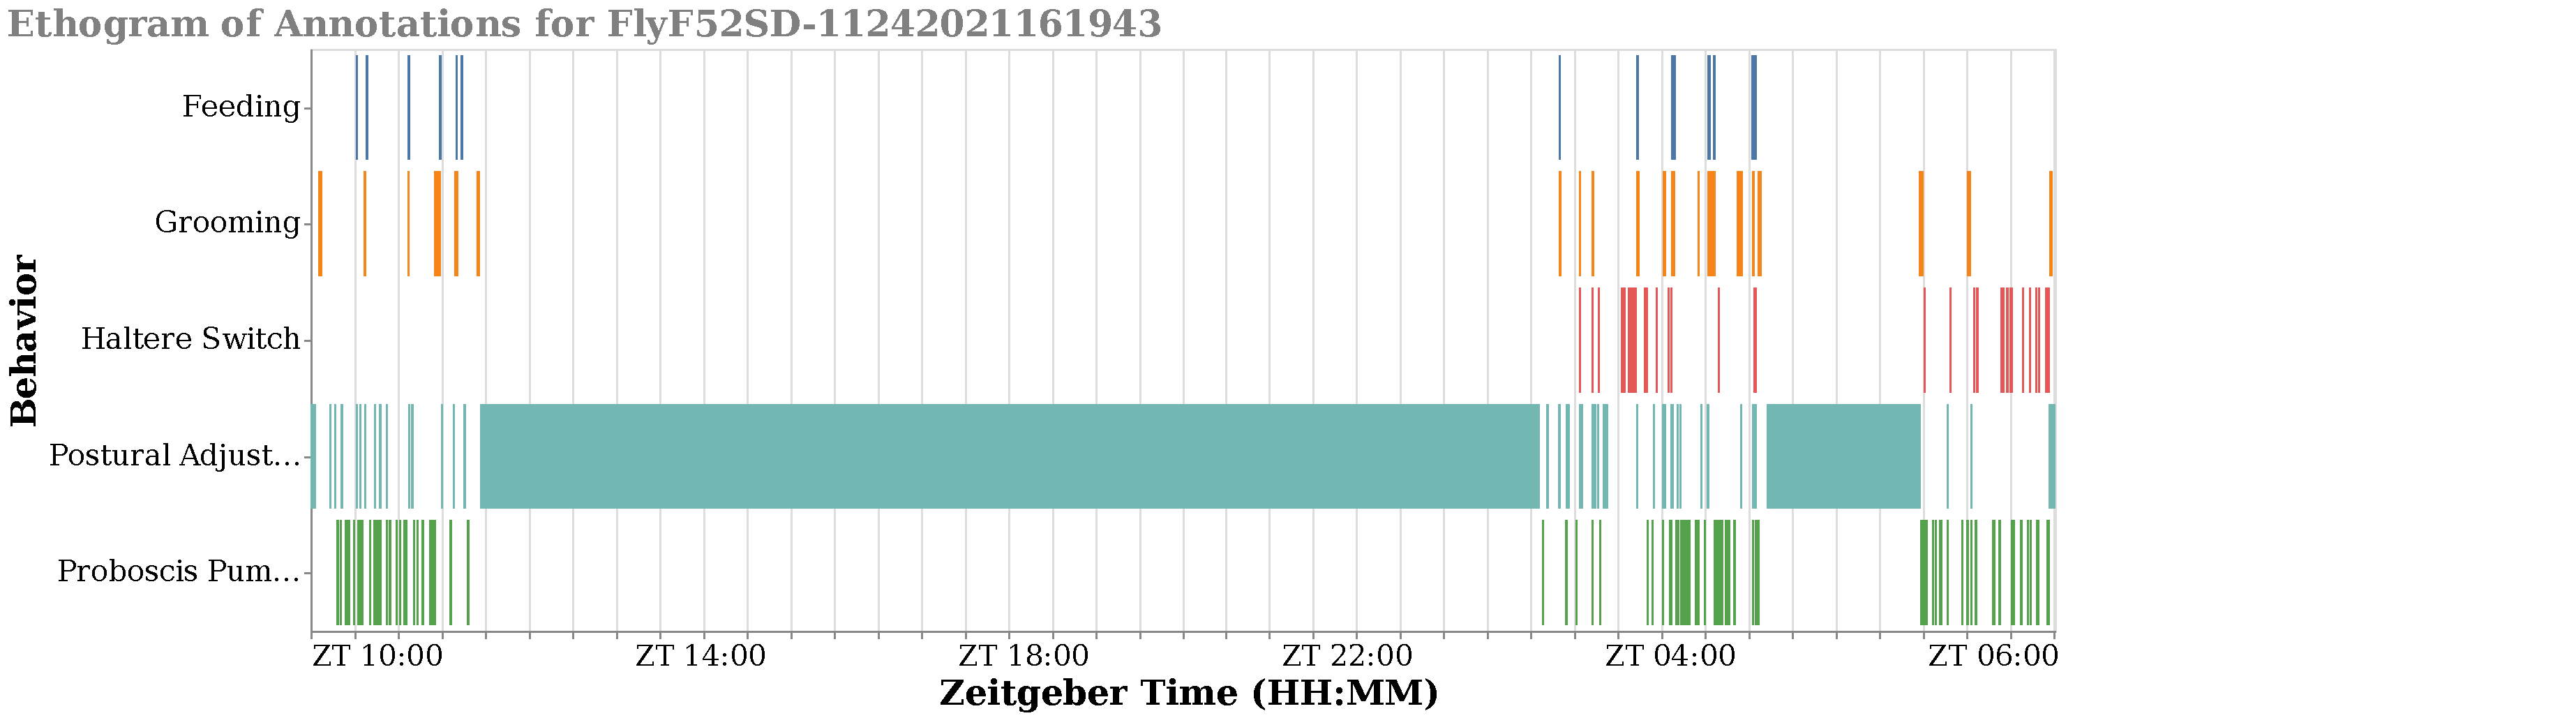
\includegraphics[width=\linewidth]{figures/FlyF52SD-11242021161943_annotation_ethogram.pdf}
		\caption{Sleep deprived.}
	\end{subfigure}%
	\caption[Two example ethograms of annotated behaviors observed during the sleep experiments.]{Two example ethograms of annotated behaviors observed during the sleep experiments. Dark period starts at ZT 12, and ends at ZT 0.}
\end{figure}
